\documentclass[a4paper,12pt, oneside, titlepage]{book}
\usepackage[romanian]{babel} % choose the language
\usepackage[utf8]{inputenc} % äöå
\usepackage[T1]{fontenc}
\usepackage[a4paper, inner=3cm, outer=3cm, top=3cm, bottom=3cm]{geometry}
\usepackage[onehalfspacing]{setspace} 
\usepackage{mathptmx} % Times New Roman
\usepackage{tikz} % Support for pictures in latex format -> convert svg files into tikz format at first
\usepackage{etoolbox} % this one makes a workaround with page numbering possible
\usepackage{csquotes} % BibLaTex stuff
\usepackage[style=verbose-ibid,backend=biber]{biblatex}
\usepackage{wrapfig}
\usepackage[export]{adjustbox}
\bibliography{chapters/references} % write your list of references into referenser.bib located in Chapters
\graphicspath{ {img/} }
% Table of contents
\setcounter{secnumdepth}{5}
\setcounter{tocdepth}{5}
\usepackage{needspace}
\usepackage[hidelinks=true,hyperindex=false,bookmarksopen=true]{hyperref}
\usepackage[cmex10]{amsmath}
\usepackage[noabbrev]{cleveref}
\usepackage{pdflscape}
\usepackage{float}
\selectlanguage{romanian}
\usepackage{amsthm}
\usepackage{caption}
\usepackage{listings}
\newtheorem{definition}{Definiţie}
\newcommand{\code}[1]{\texttt{#1}}
\Crefname{figure}{Figura}{Figuri}


\usepackage[linesnumbered,ruled,vlined]{algorithm2e}
\crefname{algocfline}{alg.}{algs.}
\Crefname{algocfline}{Algoritmul}{Algoritmi}
\SetAlgorithmName{Algoritmul}{algoritm}{Lista algoritmilor}
\begin{document}

\pagestyle{empty}    
\begingroup
\patchcmd{\chapter}{plain}{empty}{}{}

%------ Cover page stuff 

\begin{titlepage}
\thispagestyle{empty}

\mbox{}\\[6pc]
\begin{center}
	\Huge{Sistem de achiziţie, procesare si distribuite a datelor}\\[2pc]
	
	\Large{Petrişor-Ştefan Lăcătuş}\\[1pc]
	\large{Septembrie 2015}\\[2pc]
	
	Automatică şi Ingineria Sistemelor\\
Facultatea de Automatica si Calculatoare
\end{center}
\vfill

\noindent Coordonator: Ş.L. Andreea Udrea

\end{titlepage}

%------ end of cover page stuff

\tableofcontents 

\endgroup % end of TeX group

\clearpage
\pagestyle{plain}      
\pagenumbering{arabic} % Page numbering starts from here

% Example of structure

\chapter{Introducere}

Într-o lume emergenta, a dispozitivelor inteligente şi cu puternice capabilităţi de conectare, problema folosiri în mod corect şi eficient a datelor devine din ce mai importantă. Mai mulţi analişti în domeniu estimează creşteri ameţitoare ale numărului de dispozitive: $5*10^9$ până în 2020 şi $10^{12}$ până în 2035 \autocite{iotGrowth}. Deşi aceste estimări sunt foarte apropiate de certitudini, ce este însă neclar, este modul în care aceste dispozitive vor fi folosite pentru a realiza aplicaţii conectate, care înglobează uniform date din sisteme complet diferite.

Problema poate fi generalizată în următoarele trei concepte:
\begin{itemize}
	\item  \textbf{Colectarea de date:} Tot mai multe dispozitive folosesc volume mari de date în formate variate. Aceste date trebuie stocate în mod eficient folosind instrumente de stocare scalabile. 
	\item \textbf{Prelucrarea datelor}: Date din surse variate trebuie combinate pentru a obţine informaţii. Aici sunt incluse atât datele stocate local, cât şi date disponibile din alte sisteme şi servicii ce trebuie interogate. Din aceste date se urmăreşte generarea de date noi, cu valoare şi semnificaţie mai mare.
	\item \textbf{Conectarea}: Datele procesate trebuie făcute accesibile pentru sisteme exterioare.
\end{itemize}

Problema aceasta se întâlneşte atât în mediile industriale, cât şi în aplicaţiile de mici dimensiuni. 
În ultimii 5 ani, a avut loc o noua revoluţie industrială \autocite{ptc} . Paradigma industrială clasică este înlocuită la o paradigmă nouă în care procesele de fabricaţie sunt digitalizate complet, toate componentele procesului de fabricaţie fiind conectate central \autocite{deloitteReport}. 
Tradiţional, această interconectare se face prin intermediul automatelor programabile, conectate la un sistem de tip SCADA. Această structură are totuşi dezavantajul ca este statică şi nu valorifică în totalitate existenţa unor senzori inteligenţi, iar fiecare automat trebuie programat individual pentru un singur scop, datele achiziţionate fiind greu de centralizat.

Pe de altă parte, pentru aplicaţiile din mediul privat, sistemele care centralizează şi procesează datele sunt fie foarte scumpe, restricţionând utilizatorul la senzori şi dispozitive produse de un singur producător, fie sunt greu de configurat, necesitând multe echipamente separate de procesare. Spre exemplu, o automatizare a casei, folosind echipamente Siemens, costa aproximativ 15000\euro, dispozitivele de procesare reprezentând jumătate din acest preţ. Pe de alta parte, pachete software open-source, precum OpenHAB \autocite{openHab} rezolvă un subset al problemei, uşurând integrarea echipamentelor compatibile, însă nu sunt destul de generice, având aplicabilitate într-un singur domeniu.

Soluţia propusă doreşte să răspundă la problema aplicaţilor de dimensiuni mici şi mijlocii, în special din mediul privat care, propunând o alternativă la achiziţionarea de PLC-uri sau alte dispozitive complicate pentru stocarea şi procesarea datelor. Aceasta unifică achiziţia, procesarea, stocarea şi distribuţia datelor într-o singura aplicaţie ce poate fi instalată atât local, cat şi pe o instanţă cloud, permiţând accesul din orice locaţie. Un alt avantaj al unificării tuturor acestor funcţionalităţi într-o singură aplicaţie este prezentarea unui interfeţe standard pentru implementarea proceselor de procesare. Astfel, se evită unul din cele mai mari avantaje ale automatelor programabile, la care, fiecare producător are propriile standarde de implementare a aplicaţiilor.

Una din cerinţele iniţiale pe care aplicaţia a urmărit să le respecte este aspectul generic a datelor. Deşi majoritatea aplicaţiilor vor fi în procesarea numerică, acesta este doar unul din mai multe tipuri de date. Acest aspect generic permite folosirea soluţiei ca o magistrală de procesare a datelor în medii de lucru, care transformă date complexe produse de un sistem în date ce pot fi acceptate de alt sistem, menţinând un istoric în tot acest timp.

Următoarele funcţionalităţi sunt incuse în aplicaţie:
\begin{itemize}
	\item Colectarea datelor de la dispozitive şi servicii.
	\item Implementarea funcţiilor de procesare folosind limbaje de nivel înalt.
	\item Realizarea procesării folosind diagrame funcţie bloc.
	\item Posibilitatea de integrare în alte sisteme.
	\item Monitorizarea în timp real.
\end{itemize}

Lucrare urmăreşte prezentarea implementării acestei soluţii. \Cref{chapter:arhitecture} prezintă arhitectura generală, descriind entităţile folosite şi modul în care acestea interacţionează. \Cref{chapter:interfata} ilustrează interfaţa vizuală pe care aplicaţia o pune la dispoziţia utilizatorului, iar \cref{chapter:implemetare} descrie în detaliu implementarea. Ultimele două capitole, \ref{chapter:studiuCaz} şi \ref{chapter:concluzii}, prezintă un caz de utilizare al aplicaţiei respectiv câteva concluzii şi dezvoltării ce ar putea îmbunătăţi soluţia propusă.

\chapter{Arhitectura soluţiei}
\label{chapter:arhitecture}
\newlength{\bulletwidth}\settowidth{\bulletwidth}{$\bullet$}
\newcommand{\mitem}{\setlength{\leftskip}{\leftmargin}\hspace*{-\labelsep}\hspace*{-\bulletwidth}$\bullet$\hspace*{\labelsep}}
\newcommand{\mend}{\setlength{\leftskip}{0cm}}
\section{Prezentare generală}
Sistemul de achiziţie, procesare şi distribuţie a datelor a fost conceput ca o platformă de dezvoltare rapidă, bazat pe modele. Utilizatorul poate să îşi concentreze resursele asupra soluţiei finale, abstractizând detaliile implementării prin folosirea unor metode de programare vizuală, cu blocuri refolosibile în mai multe aplicaţii diferite. 
Aplicaţia a fost construită pe baza unei arhitecturi modulare; modulele fiind cât mai puţin interconectate, permiţând modificări rapide şi testarea modulelor individual. Urmărind această gândire modulare s-au identificat 4 componente esenţiale: 
\begin{itemize}
	\item \textbf{Baza de date} Asigură stocarea datelor şi a entităţilor existente;
	\item \textbf{Interfaţa web pentru management} O interfaţă uşor de utilizat ce permite  utilizatorului să manipuleze canale, diagrame, blocuri de procesare, dar şi alţi utilizatori
	\item \textbf{API-ul pentru date} Un API specializat în achiziţia de  date şi care permite informarea altor dispozitive cu privire la apariţia unor date noi.
	\item \textbf{Elemente de procesare} Asigură procesarea datelor, atât în cadrul blocurilor de procesare, cât şi în cadrul diagramelor funcţionale.
\end{itemize}
\begin{figure}
	\centering
	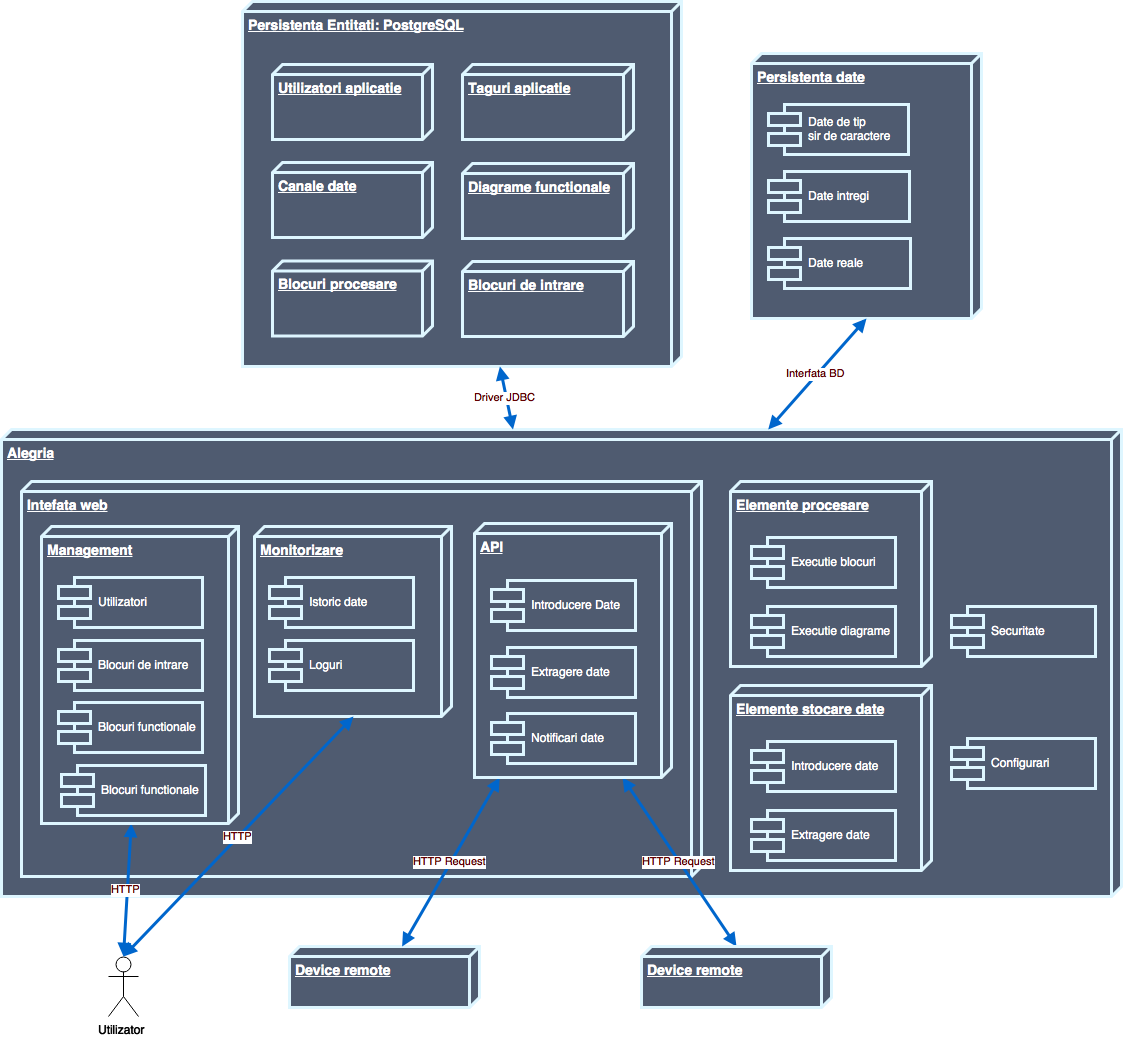
\includegraphics[width=1.3\textwidth, center]{arhitecturaGenerala}
	\caption{Arhitectura generală a aplicaţiei}
	\label{fig:arhitecture}
\end{figure}

În vederea implementării sistemului s-au identificat următoarele elemente componente esenţiale, componente ce reprezintă elementele constructive a sistemului. Acestea au reprezentare atât în baza de date, ca entităţi, cât şi în aplicaţia Java, ca clase. Identificarea acestor elemente s-a făcut pe baza analizei cazurilor de utilizare ale produsului în care s-au investigat metodele prin actorii interacţionează cu sistemul.
\begin{itemize}
	\label{list:entities}
	\item \textbf{Canalul de date} Reprezintă elementul de bază a sistemului ce asigură recepţia, persistenţa şi emiterea de date.  La crearea canalului, datele dintr-un canal, trebuie să respecte un format prestabilit. Pentru transformarea datelor în formatul stabilit se poate introduce un bloc de pre-procesarea care transformă datele din formatul brut în formatul standard;
	\item \textbf{Blocul de intrare} Elementul ce mapează un element din lumea reală în interiorul platformei. Blocurile de intrare permit gruparea mai multor canale de date într-o structura unică;
	\item \textbf{Blocul de procesare} Elementul dinamic al aplicaţiei ce aplică transformări asupra datelor. Un bloc de procesare primeşte ca intrări mai multe canale de date şi are la ieşire un alt canal de date. Utilizatorul poate folosi blocuri standard, existente în sistem, sau poate implementa blocuri noi direct în interfaţa programului;
	\item \textbf{Diagrama funcţie bloc(FBD)} Foloseşte blocuri de intrare, canale de date şi blocuri de procesare pentru a descrie o funcţie complexă cu 0-n intrări şi o ieşire. Aceste diagrame folosesc datele - aflate pe canalele de date - ce sunt trimise către blocurile de procesare şi la final se obţine un singur rezultat care este salvat pe un canal de date.
\end{itemize}

\subsection{Baza de date}

Fiind vorba despre o aplicaţie puternic bazata pe date, aceasta are nevoie de un nivel de persistenţă de înaltă performaţă. 
Urmărind arhitectura propusă din \cref{fig:arhitecture}, putem identifica două cazuri de utilizare pentru baza de date: 
\begin{itemize}
	\item Stocarea modelului entităţilor: fiecare entitate descrisă în lista de mai sus trebuie stocată în baza de date, într-o structură relaţională. Entităţile sunt puternic interconectate şi de aceea este recomandată o bază de date relaţională, de tip SQL. 
	Din punct de vedere al dimensiunii setului de date, chiar şi în aplicaţiile de mare complexitate, este vorba despre câteva milioane de înregistrări. Factorul care face acest număr să crească este conectarea a tot mai multor dispozitive, ce duce la din ce în ce mai multe canale de date. Astfel, stocarea entităţilor nu va aduce probleme de performaţă. 
	\item Stocarea datelor: în baza de date vor fi stocate atât datele primite pe fiecare canal asociat unui bloc de intrare, cât şi datele procesate de diagrame. Aceste date au un puternic caracter istoric, reprezentând o serie de timp în care se reţine  valoarea fiecărui punct de date la un anumit moment. Problema stocării acestor date este una mai complicată datorită necesităţii unei puternice scalari a bazei de date. Această problemă reprezintă un caz de utilizare pentru o baza de date NoSQL sau chiar o bază de date specializată în stocarea seriilor de timp \autocite{openTSDB}.  
\end{itemize}

\subsection{Aplicaţia Java}
Legătura dintre baza de date şi utilizatorii finali se face prin intermediul unei aplicaţii Java complexe, care este obiectul acestui proiect. Aplicaţia conţine toată logica platformei, de la operaţii asupra entităţilor din baza de date, la adăugarea,  extragerea şi procesarea datelor. 
Separarea modulelor s-a făcut pe baza scopului acestora astfel:
\begin{itemize}
	\item \textbf{Administrare}: pentru administrarea entităţilor din baza de date. Aceste module permit atât operaţii de căutare şi afişare, cât şi de creere, editare şi ştergere a utilizatorilor, a blocurilor de intrare şi funcţionale, şi a diagramelor. Fiecare dispune de o interfaţă HTML5;
	\item \textbf{Monitorizare}: permite monitorizarea execuţiei aplicaţiei de la vizualizat loguri pentru a diagnostica probleme până la realizarea de grafice folosind datele de pe anumite canale. Tot aici este disponibilă şi funcţia de a exporta date în formate uzuale (CSV, fişiere Microsoft Excel, etc);
	\item \textbf{API}: aplicaţia dispune şi de un API pentru a fi folosit programatic de către alte aplicaţii externe. Acesta este format din două componente: servicii pentru administrarea entităţilor şi servicii pentru adăugarea şi extragerea datelor;
	\item \textbf{Elemente de procesare}: sunt împărţite în două subcategorii: cele pentru procesarea blocurilor de intrare şi de procesare, şi cele pentru procesarea diagramelor;
	\item \textbf{Elemente stocare date}: permit interfaţarea cu sursele de date. Prin intermediul unei interfaţe abstractă, acestea asigură servicii de introducere şi extragere a datelor care nu ţin cont de modul în care baza de date este implementată;
	\item \textbf{Alte module}: asigură, printre altele securitatea aplicaţiei.
\end{itemize}

\section{Entităţi}
\subsection{Punctul de date}

Punctul de date reprezintă elementul constructiv al sistemul reprezentând obiectul procesării, stocării şi distribuţiei. 

Sistemul acceptă intern date în următoarele formate, ilustrate şi în \cref{fig:dataType}: 

\mitem \textbf{Long}: numere în intervalul $(-2^{63}, 2^{63} -1)$, fără virgulă; foloseşte \code{Long};
\begin{wrapfigure}{r}{0.38\textwidth}
	\centering
		\captionsetup{justification=centering}
	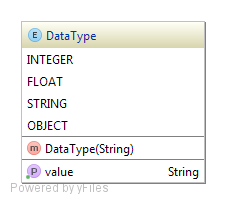
\includegraphics[width=0.38\textwidth]{dataType}
	\caption{Tipurile de date acceptate în sistem}
	\label{fig:dataType}
\end{wrapfigure}
\mitem \textbf{Real}: numere cu virgulă, având dublă precizie, reprezentate pe 64-bit conform standardului \autocite{4610935} IEEE 754;  foloseşte \code{Double} pentru reprezentare internă;

\mitem \textbf{Sir de caractere}: Un şir de caractere fără lungime limită ce trebuie formatat conform \autocite{rfc4627}. 

\mitem \textbf{Obiect}: Un obiect Java serializat în text. Intern, asemănător cu tipul de date String. 
\mend
\\
\\
\begin{figure}[h]
	\centering
	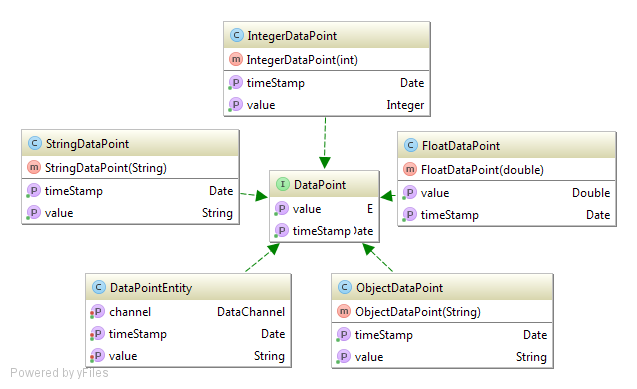
\includegraphics[width=1.1\textwidth, center]{dataPoint}
	\caption{Clasele care implementează interfaţa DataPoint}
\end{figure}

\subsection{Canalul de date}

Canalul de date este entitatea care asigură "curgerea" datelor prin sistem. Orice punct de date din sistem aparţine unui canal, acest lucru fiind realizat drept constrângere atât la nivelul aplicaţiei, cât şi la nivelul bazei de date.
\begin{figure}[H]
	\centering
	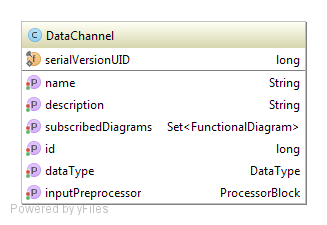
\includegraphics[width=0.55\textwidth]{dataChannel}
	\caption{Clasa DataChannel}
\end{figure}

Canalul de date este şi mijlocul prin care utilizatorul interacţionează cu punctele de date. Când un dispozitiv adaugă date noi în sistem, acestea sunt ataşate unui canal  care poate fi folosit ca una dintre intrările unei diagrame de blocuri funcţionale. De asemenea, datele procesate de o diagramă sunt ataşate unui canal permiţând apoi accesul pentru extragerea datelor deja existente şi pentru a primi notificări de fiecare dată când pe un canal apar informaţii noi.

În plus, un canal de date poate avea şi un bloc de preprocesare ataşat. Acesta este executat de fiecare dată când date noi încearcă să fie introduse în canal, permiţând validarea şi transformarea datelor brute în date ce respectă tipul de date al canalului.  
\subsection{Blocul de intrare}
Blocurile de intrare modelează elemente reale din aplicaţie, grupând mai multe canale de date şi expunându-le pentru a permite introducerea datelor din exterior. Acestea descriu modul în care datele sunt legate de un element real. 

[iulia]Spre exemplu, o sursă inteligentă si conectată in alimentare neîntreruptibilă din \cref{fig:ups} poate fi privită ca un bloc de intrare, unde fiecare senzor este reprezentat de un canal de date. [iulia] Dispozitivul inteligent devine astfel conectat la platforma şi poate trimite date către aceasta. Pentru că datele pot avea perioade de eşantionare diferite, dispozitivul trimite date de la unul sau mai mulţi senzori odată, fiecare canal de date fiind tratat individual.

Un alt mod în care blocurile de intrare pot fi privite este ca obiecte, sau "Things" în cadrul Internetului Tuturor Lucrurilor (Internet of Things - IoT). Astfel, putem privi blocurile de intrare ca dispozitive ce monitorizează bătăile inimii sau activitatea celebrară, ca automobile cu reţele complexe de senzori, sau chiar aplicaţii de lucru ce generează date în timp real. Prin acest mijloc, dispozitive inteligente se pot conecta în platformă, fie trimiţând direct date, fie prin intermediul unui agent care se află pe dispozitiv, agent ce funcţionează ca un \textit{gateway}, implementând protocoale de comunicaţie proprietare.

\begin{figure}[H]
	\centering
	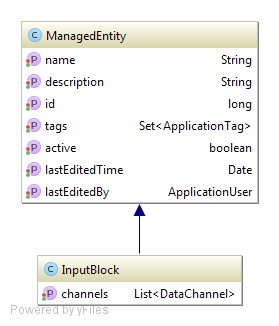
\includegraphics[width=0.55\textwidth]{inputBlock}
	\caption{Clasa \textbf{InputBlock}}
\end{figure}
\begin{figure}[H]
	\centering
	\includegraphics[width=\textwidth]{UPS}
	\caption{Modelarea unui UPS inteligent în Alegria}
	\label{fig:ups}
\end{figure}

\subsection{Blocul de procesare}

Blocurile de procesare realizează operaţiile de transformare a datelor. Din punct de vedere funcţional, acestea au la intrare ultimele date introduse de pe mai multe canale şi returnează un singur punct de date, comportându-se ca un element de tip "black-box"\autocite{functionBlocks}. Pentru implementare, utilizatorul foloseşte limbaje dinamice, precum JavaScript sau Ruby, scriind cod direct în interfaţa web. Acest cod este rulat de către server. 
Conceptul de blocuri de procesare reprezintă o implementare a blocurilor de operaţii definite în standardul  IEC61131-3 \autocite[Apendix C]{IEC61131-3} .

Blocuri pre-implementate, existente în orice instantă a platformei, permit rezolvarea de probleme complexe cu cunoştinţe minime de programare.
Un alt aspect important al blocurilor de procesare, este faptul ca sunt independente de sursa de date, ele oferind doar mijloace de prelucrare a unor date abstracte. Această abstractizare permite refolosirea lor în mai multe proiecte. Spre exemplu, un bloc care face media tuturor intrărilor nu ţine cont de originea datelor. 

Blocurile \textbf{nu au memorie statică}. Ele pot folosi informaţii exterioare, cum ar fi timpul curent al zilei sau alte informaţii din sistem, sau pot chiar accesa servicii web, însa ele nu au stare interioară. Astfel, se poate considera că blocurile reprezintă un element combinaţional şi nu unul secvenţial.
\begin{figure}[H]
	\centering
	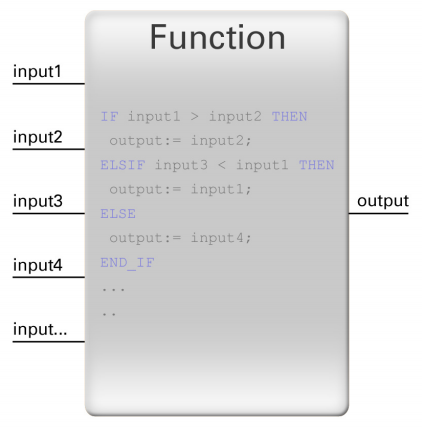
\includegraphics[width=0.55\textwidth]{exempluBlock}
	\caption{Exemplu bloc de procesare}
\end{figure}

\begin{figure}[H]
	\centering
	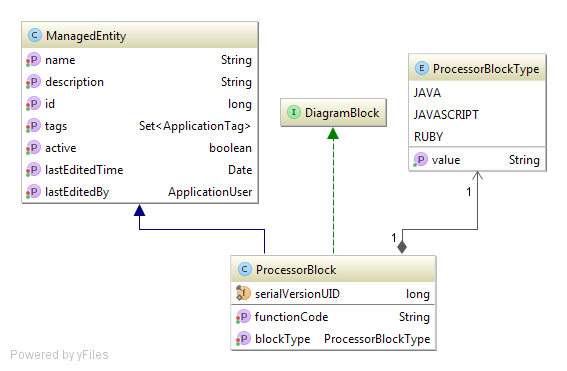
\includegraphics[width=\textwidth]{processorBlock}
	\caption{Clasa \textbf{ProcessorBlock}}
\end{figure}

\subsection{Diagrama funcţie bloc (FBD)}

Diagramele funcţie bloc reprezintă o implementare a unuia din cele patru limbaje de programare pentru automate programabile, specificate de standardul IEC 61131-3:2013 \autocite[128-140]{IEC61131-3}. FBD reprezintă un limbaj de control al procesului, iar, în mod normal, toate blocurile de procesare dintr-o diagrama sunt executate.
În cel mai simplu caz de utilizare, o FBD realizează următoarele operaţii:
\begin{itemize}
	\item Acceptă date de intrare de la unul sau mai multe canale;
	\item Realizează o operaţie de transformare asupra acelor date folosind un bloc de procesare;
	\item Salvează rezultatul pe un canal de ieşire.
\end{itemize}
Legăturile dintre blocuri sunt unidirecţionale. Un bloc de procesare poate trimite rezultatul său la unul sau mai multe blocuri, iar o intrare poate fi conectată la o singură ieşire. Transmiterea de date se face fără întârzieri. Diagramele sunt executate în ordinea definită de ordonarea topologică a nodurilor din graful ce defineşte diagrama \autocite[20-50]{IEC61499}. 
\begin{figure}[H]
	\centering
	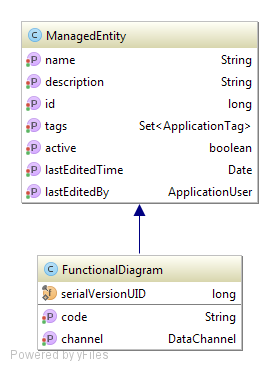
\includegraphics[width=0.5\textwidth]{functionalDiagram}
	\caption{Clasa \textbf{FunctionalDiagram}}
\end{figure}

\begin{figure}[H]
	\centering
	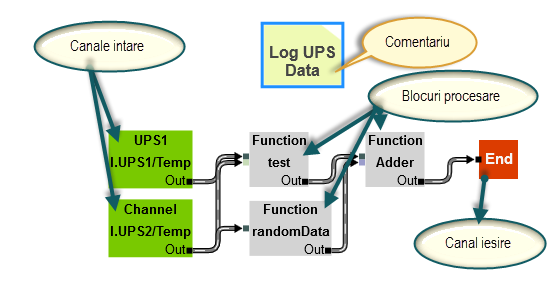
\includegraphics[width=0.95\textwidth]{exempluDiagrama}
	\caption{Exemplu diagrama funcţională}
	\label{fig:exempluDiagrama}
\end{figure}

\section{Primirea datelor}
Primirea datelor se face prin intermediul unei interfeţe de transfer a stării (REST). Pentru integrarea mai uşoară cu sisteme deja existente sunt acceptate mai multe formate. Astfel, au fost implementate mai multe procesoare care primesc date atât într-un format nou, caracteristic aplicaţiei, cât şi în formate standard din industrie.
În această versiune, modalităţi de trimitere a datelor au fost implementate:
\begin{itemize}
	\item Trimitere către un singur canal, un singur punct odată, pe baza serviciului\\ \textit{/api/put/{inputId}/{channelId}/{data}}. Acest serviciu adaugă un singur punct în baza de date, la momentul curent şi este folosit pentru sisteme care trimit date rar şi nu trebuie să se ţină cont de data locala de pe device-ul care a trimis punctul de date.
	\item În formatul standard folosit de openTDSB, cu următoarele modificări care păstrează totuşi compatibilitatea: metricile reprezintă numele canalului, iar tag-urile sunt opţionale. Se acceptă atât formatul în care într-o cerere se află un singur punct, cât şi formatul cu o listă de puncte. Canalele dintr-o cerere multidimensională nu trebuie să facă parte din acelaşi bloc de intrare. Acest mod de introducere a datelor este sugerat pentru sistemele care folosesc mai multe canale de date şi care trimit seturi de date mai mari printr-o singură cerere. Spre exemplu, un dispozitiv poate trimite date de pe mai multi senzori şi poate stoca local mai multe măsurători pe acelaşi senzor pentru a trimite toate datele odată.
\end{itemize}
Odată primite, noile puncte de date trec prin procesul descris în \cref{fig:intrareDate}:
\begin{enumerate}
	\item Se interoghează baza de date pentru detalii privind canalul ce tocmai a primit date.
	\item Dacă un preprocesor există pe canalul specificat, atunci el este încărcat.
	\item Se execută preprocesorul cu punctul de date primit.
	\item Se salvează rezultatul în baza de date.
	\item Asincron, se lansează toate diagramele care trebuie să se execute atunci când se primesc date noi pe acest canal.
	\item Asincron, se informează "ascultătorii" de primirea unor date noi de către canal.
\end{enumerate}
\begin{landscape}
	\begin{figure}
		\centering
		\includegraphics[width=1.7\textwidth]{introducereDate}
		\caption{Diagrama de secvenţe pentru introducerea de noi date şi execuţia diagramelor}
		\label{fig:intrareDate}
	\end{figure}
\end{landscape} 

\chapter{Interfaţa aplicaţiei}
\label{chapter:interfata}

Aplicaţia dispune de o interfaţă modernă şi a fost implementată folosind standardul HTML5, cu pagini dinamice care păstrează starea în client, prin încărcarea asincrona a elementelor. Întreaga interfaţă este de tip responsive, scalându-se automat pentru afişare pe dispozitive cu rezoluţii diferite (monitor,  tabletă sau telefoane).

La accesarea aplicaţiei, utilizatorul este întâmpinat de interfaţă de autentificare din \cref{fig:login}. 
\begin{figure}[H]
	\centering
	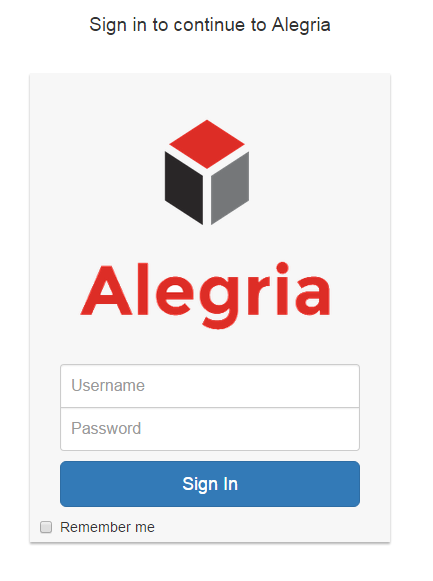
\includegraphics[width=0.5\textwidth]{screens/login}
	\captionsetup{justification=centering}
	\caption{Autentificarea în aplicaţie}
	\label{fig:login}
\end{figure}
Login-ul în aplicaţie permite accesul la interfaţa de management şi monitorizare. Navigaţia se face printr-un meniu aflat în antetul paginii, vizibil în \cref{fig:navMenu}
\begin{figure}[H]
	\centering
	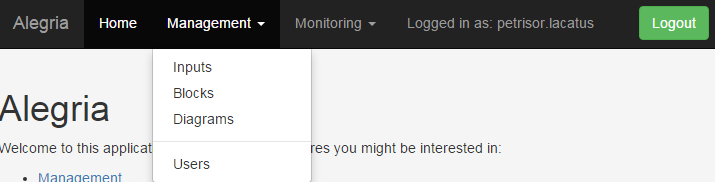
\includegraphics[width=\textwidth]{screens/navMenu}
	\captionsetup{justification=centering}
	\caption{Navigarea prin funcţiile aplicaţiei}
	\label{fig:navMenu}
\end{figure}
Dacă utilizatorul este administrator, atunci el poate accesa şi administrarea utilizatorilor. Aici el poate adăuga noi utilizatori, modifica utilizatorii existenţi sau poate dezactiva accesul unora din aplicaţie.
\begin{figure}[H]
	\centering
	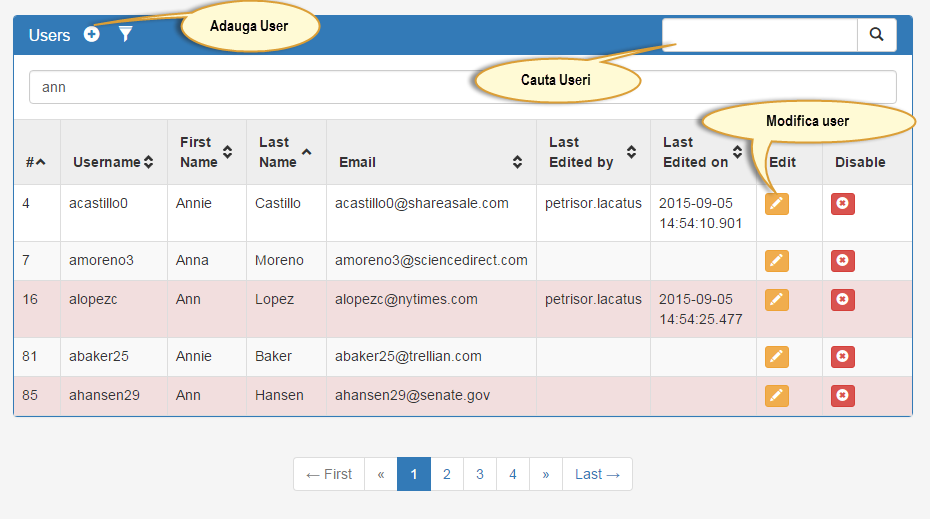
\includegraphics[width=1.2\textwidth, center]{screens/userManagement}
	\captionsetup{justification=centering}
	\caption{Managementul utilizatorilor din aplicaţie}
	\label{fig:userManagement}
\end{figure}
Toate entităţile dispun de o interfaţă similară cu cea din \cref{fig:userManagement}, în care utilizatorul are acces facil la entităţile existente în sistem. Tabelele în care datele sunt afişate permit sortarea şi filtrarea, uşurând astfel găsirea entităţii ce trebuie modificată. În plus, căutarea se poate face nu doar după numele entităţii, ci şi după taguri sau descriere. Conţinutul este paginat astfel încât timpul de încărcare a paginii să fie cât mai mic.

În cazul administrării blocurilor de intrare, un panou modal, încărcat dinamic, este disponibil pentru adăugare şi editare. În acest panou, utilizatorul poate seta taguri şi administra canalele de pe acel bloc.
\begin{figure}[H]
	\centering
	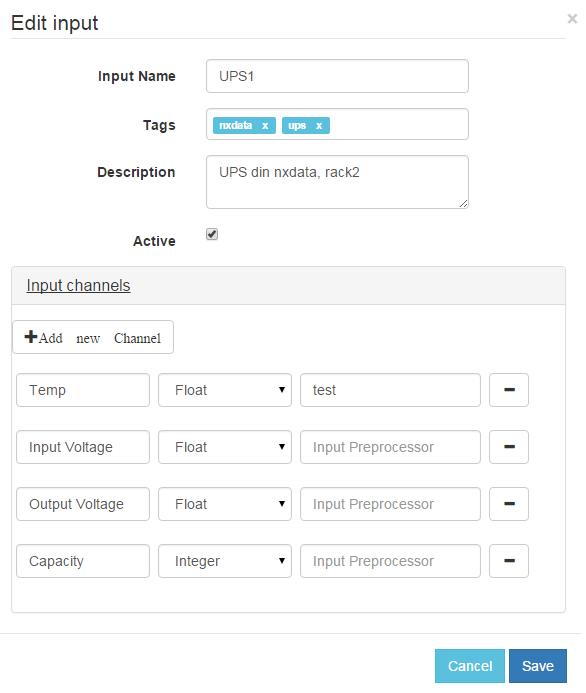
\includegraphics[width=\textwidth]{screens/inputBlock}
	\captionsetup{justification=centering}
	\caption{Editarea unui bloc de intrare}
	\label{fig:inputBlock}
\end{figure}

Pentru management-ul blocurile de procesare, utilizatorul are la dispoziţie şi un editor inteligent care afişează codul colorat în funcţie de limbajul selectat. Astfel, utilizatorii pot depista erorile de sintaxa în timpul editării codului.
\begin{figure}[H]
	\centering
	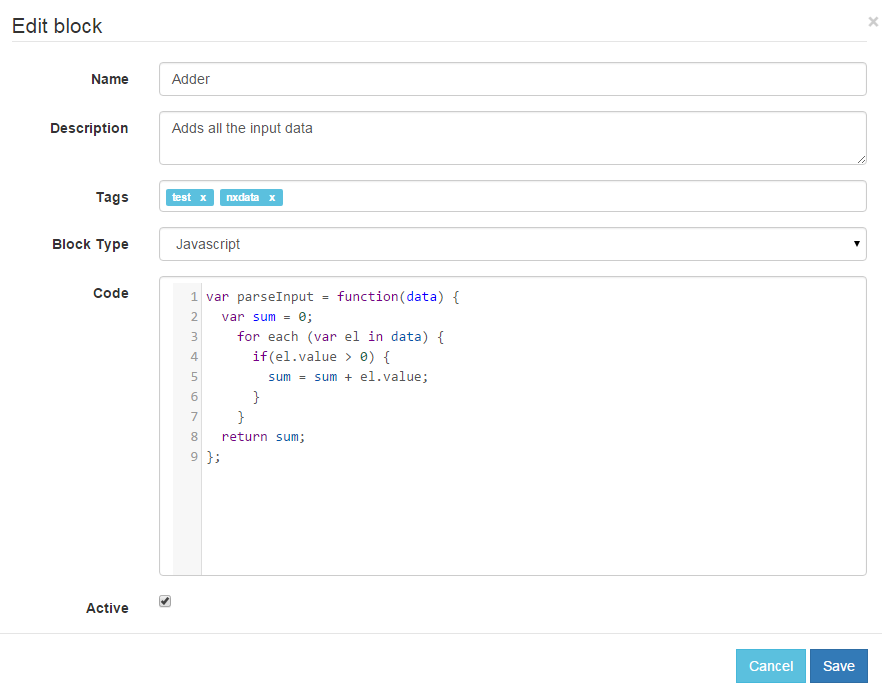
\includegraphics[width=1.1\textwidth, center]{screens/blockManagement}
	\captionsetup{justification=centering}
	\caption{Modificarea unui bloc de procesare şi editarea codului}
	\label{fig:blockManagement}
\end{figure}
Editarea diagramelor funcţionale se face vizual, într-o interfaţă asemănătoare cu cea din SimuLink sau LOGO! Soft Comfort. Aceasta interfaţă permite adăugarea vizuală a blocurilor dintr-o paletă, căutarea automată a instantelor de blocuri şi exportarea schemei diagramei pentru salvare într-un mediu extern. 

Blocurile pot fi modificate atât prin schimbarea proprietăţilor acestora din meniul ce apare în partea de jos a diagramei când blocul este selectat, dar şi direct prin acţiunea de click stânga sau dreapta pe acesta. Pentru blocurile de procesare, utilizatorul are opţiunea să vizualizeze şi să modifice codul direct din aceasta pagină, fără a mai naviga spre pagina de administrare a blocurilor de procesare.
Alături de câmpul de descriere, comentariile adăugate direct peste diagrama, ajută la documentarea implementării şi funcţionalităţii.
\begin{figure}[H]
	\centering
	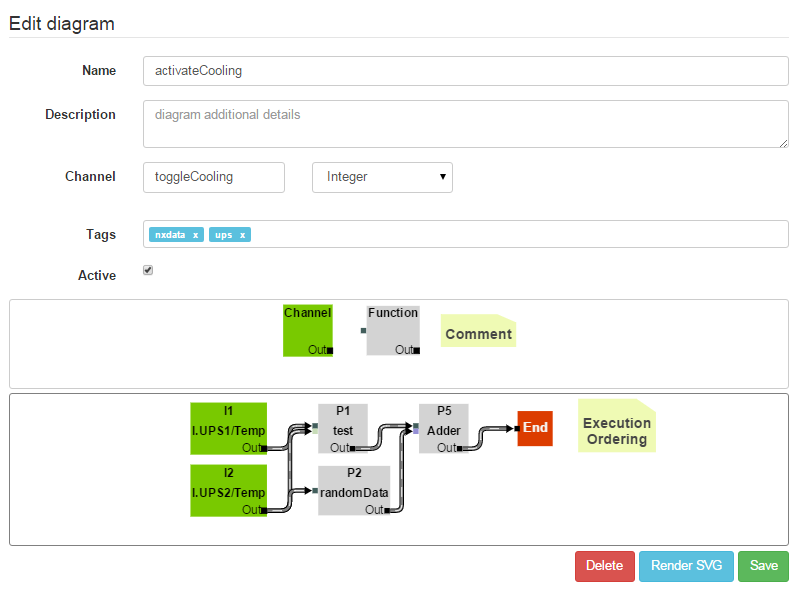
\includegraphics[width=1\textwidth, center]{screens/editDiagram}
	\captionsetup{justification=centering}
	\caption{Realizarea unei diagrame funcţionale}
	\label{fig:editDiagram}
\end{figure}

\begin{figure}[H]
	\centering
	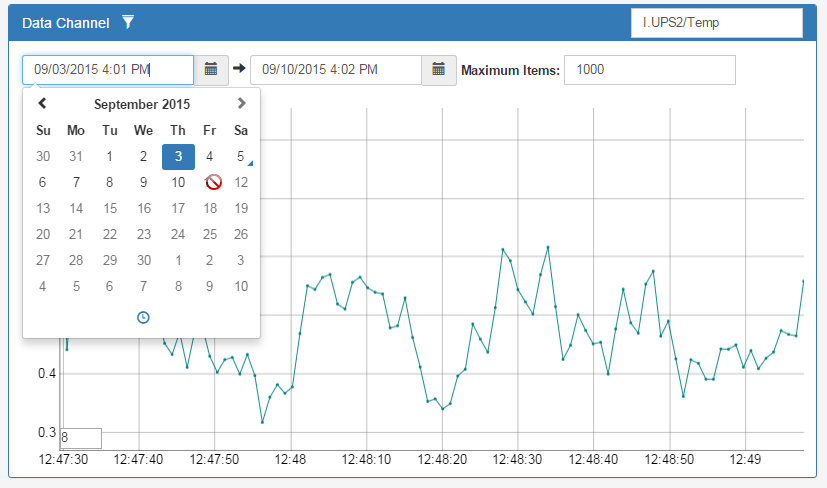
\includegraphics[width=1.1\textwidth, center]{screens/monitoring}
	\captionsetup{justification=centering}
	\caption{Monitorizarea datelor de pe un canal}
	\label{fig:monitoring}
\end{figure} 

\chapter{Implementarea aplicaţiei de achiziţie, procesare şi distribuţie a datelor (Alegria)}
\label{chapter:implemetare}
\section{Interfaţa Web}
\begin{wrapfigure}{r}{0.35\textwidth}
	\centering
	\captionsetup{justification=centering}
	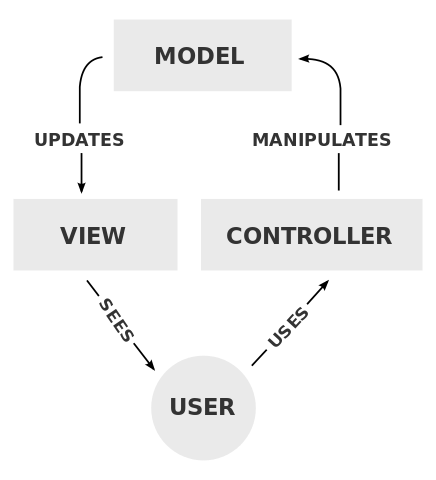
\includegraphics[width=0.35\textwidth]{mvcPattern}
	\caption{Colaborarea între componentele MVC}
\end{wrapfigure}
Aplicaţia de achiziţie, procesare şi distribuţie a datelor (Alegria) a fost implementată cu ajutorul platformei \textbf{Spring Boot} \autocite{SpringBoot}. Platforma a fost aleasă pentru stabilitatea ei excepţională, folosind Spring Framework care stă la baza unora din cele mai mari aplicaţii existente \autocite{springUseCase}, dar şi pentru uşurinţa prin care o aplicaţie poate fi compusă din elemente funcţionale, abstractizând peste nivelele de jos a programului, permiţând alocarea timpului pe logica aplicaţiei şi nu pe implementarea platformei pe care aplicaţia rulează. Un alt motiv pentru care a fost aleasă platforma Spring, este faptul că suportă programarea orientată pe aspecte şi injecţia dependinţelor, permiţând scrierea de cod curat şi uşor de testat.

Cum aplicaţia este bazată pe arhitectura MVC (model-view-controller), aceasta a fost structurată în trei elemente separate: 
\begin{itemize}
\item  \textbf{Interfaţa vizuală}: Realizată în \textbf{HTML5}, folosind motorul de templating Thymeleaf pe server şi Bootstrap cu JQuery în client pentru afişarea paginilor. Această combinaţie permite realizarea de pagini de tip responsiv, compatibile cu toate dispozitivele existente pe piaţă indiferent de rezoluţie ( monitor cu display mare, tabletă, telefon mobil, etc).

\item  \textbf{Modele}: O reprezentare a entităţilor din baza de date în sistemul de achiziţie, procesare şi distribuţie a datelor (Alegria).

\item  \textbf{Controller-e}: Realizează legătura dintre partea vizuală a aplicaţiei şi entităţile din baza de date, asigurând atât metodele care "completează" template-urile cu date, cât şi implementarea interfeţei API care introduce şi extrage date.
\end{itemize}

\subsection{Securitate}
Securitatea este un aspect foarte important ce trebuie considerat, atât pentru accesul la date, cât şi la entităţi. Astfel, în implementare s-a folosit framework-ul \textbf{Spring Security} care uşurează management-ul securităţii, fiind puternic integrat şi cu restul platformei Spring.

Pentru autentificare în vederea utilizării unei resurse protejate, utilizatorul va folosi unul din două mecanisme:
\begin{itemize}
	\item Autentificare securizată prin username şi parolă, aceste detalii fiind stocate în tabelă \textit{application\_user}, parola fiind stocată abia după ce a fost trecută printr-o funcţie criptografică de hashing. Această metodă este folosită pentru autentificarea utilizatorilor în interfaţa de management şi monitorizare. Odată ce procesul a reuşit, un token unic va fi generat, iar request-urile următoare vor fi verificate pe baza procesului descris mai jos.
	\item Autentificare pe baza de token, folosită pentru securizarea API-ului, dar şi în cazul în care un utilizator s-a autentificat deja cu username şi parolă. Fiecare request trebuie sa aibă un token, fie într-un cookie, fie ca parametru în url.
\end{itemize}
Tot în scopuri de securitate, fiecare entitate ce poate fi modificată menţine un istoric al tuturor modificărilor, împreună cu utilizatorul care le-a efectuat, iar, pentru o dezvoltare ulterioară, accesul unui utilizator poate fi limitat doar la obiectele care au aceleaşi tag-uri ca şi utilizatorul.
\begin{landscape}
	\begin{figure}
		\centering
		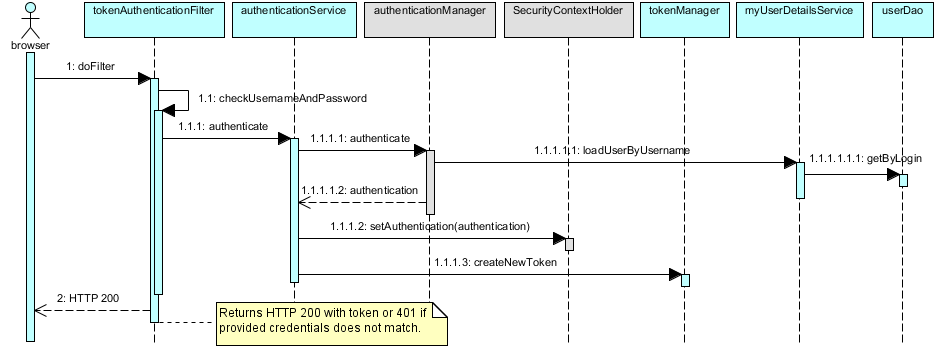
\includegraphics[width=1.75\textwidth, center]{loginUml}
		\caption{Procesul de autentificare în aplicaţie}
		\label{fig:loginUml}
	\end{figure}
\end{landscape}



\subsection{Management}
\begin{figure}[H]
	\centering
	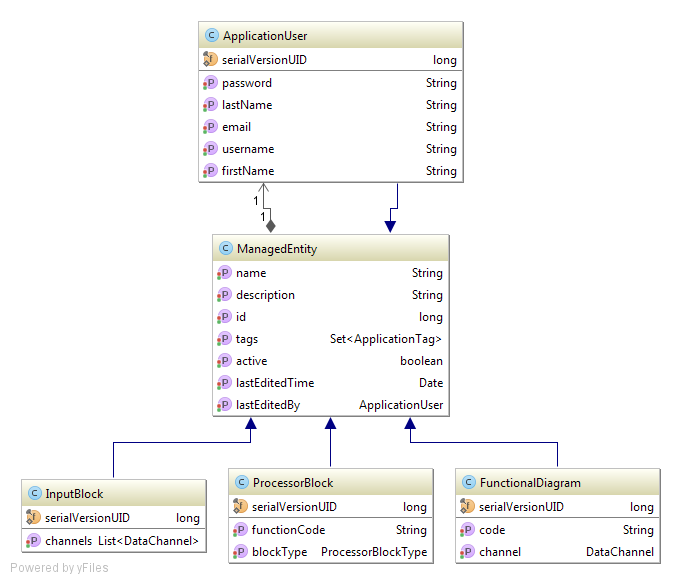
\includegraphics[width=\textwidth, center]{managedEntities}
	\captionsetup{justification=centering}
	\caption{Diagrama claselor care sunt administrate de către utilizator şi implementează \code{ManagedEntity}}
	\label{fig:managedEntities}
\end{figure}
Toate entităţile care implementează \code{ManagedEntity} permit apoi operaţii de adăugare, modificare şi ştergere. Acest proces de administrare vizuală foloseşte următoarele resurse:
\begin{itemize}
	\item Un \textbf{repository}, care extinde \code{JpaRepository} din framework-ul Spring Data. Acesta asigură operaţii de căutare, creare, citire, modificare şi ştergere a entităţilor. Un avantaj al folosirii  acestui repository, care implementează paradigma Data Acces Object (DAO) este că interacţiunea cu baza de date se face într-un mod consistent şi sigur, incompatibilităţile de tip fiind detectate la compilare, şi nu la rulare. În Alegria, toate repository-urile folosite, împreuna cu implementările lor, se află în package-ul \code{ro.pub.acse.sapd.repository}.
	\item O \textbf{vizualizare}, template Thyeleaf, care, într-o singură pagină HTML expune către utilizator toate operaţiile suportate de repository. Această pagină este dinamică, ce foloseşte dialoguri modale încărcate prin AJAX pentru a edita entităţi, fără a fi necesar ca utilizatorul sa fie redirecţionat. Entităţile sunt afişate sub forma tabelară, dinamică, care permite sortarea şi filtrarea după diverse condiţii. Dialogul modal de editare este specific entităţii modificate. Vizualizările pentru întreaga listă se află în \code{resources\textbackslash templates\textbackslash management} iar conţinutul dialogului modal se află în subdirectorul \code{fragments}.
	\item Un \textbf{controller}, clasă cu adnotarea \code{@Controller}, leagă repository-ul de vizualizare şi specifică către Spring care sunt endpoint-urile (căile pe care acest controller le tratează) prin adnotarea \code{@RequestMapping}. Controllere-le pentru managementul entităţilor se află în \code{ro.pub.acse.sapd.controller.web.management}. Un exemplu de metode care sunt tratate într-un asemenea controller se găsesc în \cref{fig:managementInputs}.
\end{itemize}
\begin{figure}[H]
	\centering
	\captionsetup{justification=centering}
	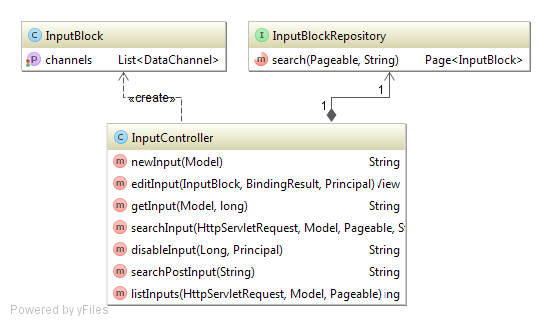
\includegraphics[width=\textwidth, center]{managementInputs}
	\caption{Interacţiunea dintre repository, controller şi entitate}
	\label{fig:managementInputs}
\end{figure}

\subsubsection{Managementul blocurilor de intrare}
Pe lângă elementele descrise mai sus, la management-ul blocurilor de intrare trebuie ca utilizatorul să poată vizualiza şi modifica lista de canale ale unui bloc. În vederea implementării acestei particularităţi, în dialogul modal pentru adăugare şi modificare, a fost realizat un formular dinamic cu câte o line pentru fiecare canal de date. Pentru blocurile de intrare care au deja un canale ataşate, acest formular este generat de către server, în template-ul thymeleaf \code{input.html}, iar, dinamismul formularului este implementat cu ajutorul unor funcţii JavaScript care manipulează structura documentului.
\begin{figure}[H]
	\centering
	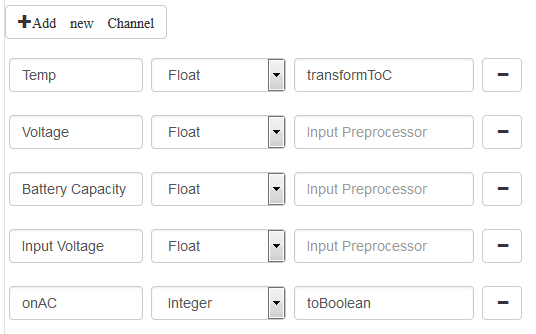
\includegraphics[width=0.8\textwidth, center]{editInput}
	\caption{Formular HTML dinamic pentru editarea canalelor unui bloc de intrare }
	\label{fig:editInput}
\end{figure}
Pentru selectarea blocului de preprocesare a fost folosit endpoint-ul din API de la adresa \code{/blocks/getBlocks} care returnează lista tuturor blocurilor de procesare în format JSON. Această listă este folosită pentru permite completarea automata a câmpului pentru blocul de preprocesare a datelor ale unui canal, folosind librăria JavaScript \textbf{Bootstrap 3 Typeahead} \autocite{typeahead}.

\subsubsection{Managementul blocurilor de procesare}
O particularitate a editării blocurilor de procesare este folosirea librăriei JavaScript \textbf{CodeMirror} \autocite{codemirror} pentru afişarea codului. Cuvintele cheie ale limbajului dat de tipul blocului fiind evidenţiate, acest lucru făcând dezvoltarea codului mult mai uşoară. Un alt avantaj al acestei librări este posibilitatea găsirii erorilor de sintaxa mult mai rapid, fără a testa blocul. Aceasta funcţionalitate este implementata cu ajutorul unei funcţii care se execută de fiecare dată când se modifică valoarea selectată în input-ul "Block Type".
\begin{figure}[H]
	\centering
	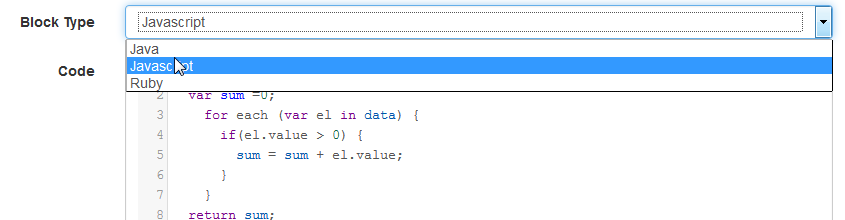
\includegraphics[width=1.2\textwidth, center]{codemirrorExample}
	\caption{Modificarea limbajului din editorul CodeMirror în funcţie de tipul blocului}
	\label{fig:codemirrorExample}
\end{figure}
\subsubsection{Managementul diagramelor}
Pentru implementarea funcţiilor de design vizual al diagramelor funcţionale s-a ales librăria JavaScript \textbf{GoJS} \autocite{gojs}. Aceasta permite implementarea de diagrame interactive, fiind compatibilă cu toate browsere-le şi cu dispozitivele mobile moderne. Librăria reprezintă un punct foarte bun de plecare deoarece asigură suport atât pentru funcţionalităţi precum drag-and-drop, copiere şi lipire, undo şi redo, şi multe alte funcţionalităţi. Un alt avantaj al acestei librării este ca suportă adăugarea de condiţii asupra diagramei chiar la construcţia acesteia. Din acest motiv, librăria a fost configurată să nu permită decât legături de la o ieşire la o intrare.

În vederea realizării acestor configurări a fost scris fişierul JavaScript \code{diagram.js}. Aici sunt configurate tipurile de blocuri:
\begin{itemize}
	\item \textbf{Canale de intrare}: acestea sunt configurate să nu poată avea intrări, ci doar o singură ieşire. Atunci când un canal de intrare este selectat, utilizatorul poate să îi atribuie un nume şi să selecteze care este canalul ce indică de acel bloc. Aceasta selecţie se face cu ajutorul unui input cu auto completare.
	\item \textbf{Blocuri de procesare}: deoarece numărul de intrări este variabil a fost implementată funcţia \code{addPort}. Aceasta este apelată atunci când utilizatorul dă click pe opţiunea "Add input" din meniul contextual al blocului. Pentru operaţiunea de ştergere a portului a fost implementată funcţia \code{removePort(port)}. Ordinea acestor porturi determină şi ordinea elementelor din lista cu care este apelat blocul de procesare. Când un bloc este selectat utilizatorul poate să îi atribuie un nume şi să indice blocul de procesare la cere se referă. Această selecţie se face cu ajutorul unui input cu auto completare. Astfel, acelaşi bloc de procesare poate fi folosit de mai multe ori chiar şi în cadrul aceleiaşi diagrame. Pentru uşurinţă dezvoltării, linkuri către detaliile blocului de procesare sunt disponibile chiar în interiorul diagramei;
	\item \textbf{Stop}: bloc ce semnifică canalul de ieşire. Configurat cu un singur port de intrare, el nu poate fi legat decât la o singura ieşire;
	\item \textbf{Comentariu}: nu se poate lega în diagramă şi nu ia parte la execuţia acesteia. 
\end{itemize}
Toate aceste blocuri sunt adăugate şi într-o paletă pentru adăugare uşoară în diagramă. Deoarece blocul "Stop" nu poate avea decât o singură instanţă, acesta nu este disponibil în paletă.
\begin{figure}[H]
	\centering
	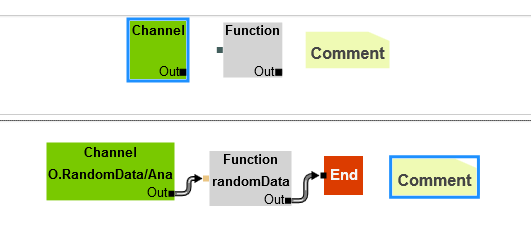
\includegraphics[width=1.2\textwidth, center]{diagramPalleteAndExample}
	\caption{Paleta de blocuri şi exemplu de instanţe ale acestora}
	\label{fig:diagramPalleteAndExample}
\end{figure}
Când utilizatorul salvează o diagramă, este generat un model JSON al acesteia, model ce este apoi salvat în baza de date. În acest model sunt salvate proprietăţile diagramei, urmate de lista nodurilor şi de legăturile dintre porturile nodurilor.

\subsubsection{Administrare tag-uri}
După cum s-a discutat în secţiunea despre securitate, fiecare entitate care este administrata de utilizator poate avea mai multe taguri. Acestea reprezintă o lista de cuvinte care specifică un concept, spre exemplu, toate entităţile care sunt folosite într-o diagrama pot avea acelaşi tag. Tagurile permit astfel gruparea entităţilor, fiind folosite în căutare.
\begin{figure}[H]
	\centering
	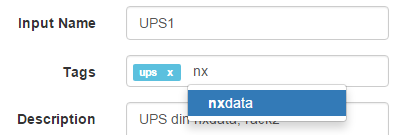
\includegraphics[width=0.7\textwidth, center]{tagsEdit}
	\caption{Editarea tag-urilor unui bloc de intrare}
	\label{fig:tagsEdit}
\end{figure}
Pentru implementare, pe partea de server au fost creata clasa \code{ApplicationTag}, cu doua câmpuri: nume, şi Id. Toate instantele acestei clase sunt salvate în baza de date, în tabela \code{application\_tag}, iar endpoint-ul \code{/tags/getTags} întoarce toate tag-urile din acea tabelă. Acest serviciu API este folosit de librăria JavaScript Bootstrap Tags Input \autocite{tagsinput}, care, împreună cu librăria de autocompletare \autocite{typeahead}, permite utilizatorului să selecteze taguri deja existente. Atunci când utilizatorul introduce totuşi un tag care nu există deja în baza de date, acesta este creat automat, fiind setat direct pe entitatea modificată. Fiecare \code{ManagedEntity} are un set de taguri, permiţând salvarea tagurilor în baza de date, într-un tabel separat, care implementeaza relaţia de tip Many-to-Many dintre entitate şi \code{ApplicationTag}.
\begin{figure}[H]
	\centering
	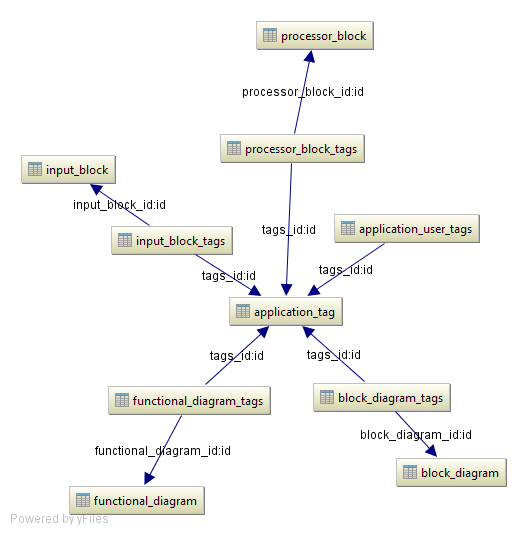
\includegraphics[width=\textwidth, center]{tags}
	\caption{Relaţiile dintre tabelă \code{tags} şi celelalte entităţi}
	\label{fig:tags}
\end{figure}
\subsection{Monitorizare}
O chestiune de mare importantă este vizualizarea datelor ce au intrat sau au fost procesate de aplicaţie. În acest scop, a fost implementată vizualizarea datelor în timp real. Pentru extragerea informaţiilor de pe un canal se folosesc endpoint-urile din API de la \code{/api/fetch/{channelId}}, care întorc punctele de pe un canal dintr-un anumit interval de timp, in format JSON.

Deoarece datele procesate de aplicaţie sunt de mai multe tipuri, apare totuşi problema modului de afişare. În funcţie de datele întoarse prin API se selectează unul din două moduri. Pentru datele numerice se foloseşte o reprezentare grafică, folosind librăria dygraphs \autocite{dygraphs}, iar pentru datele care nu pot fi reprezentate numeric, se foloseşte sunt afişarea sub formă de tabel, ca şiruri de caractere.

Pentru ambele moduri de reprezentare, utilizatorul are opţiunea să obţină doar datele dintr-o anumită perioada de timp sau ultimele înregistrări pe acel canal. Acest mod de selecţie este ilustrat în \cref{fig:monitorDataFilter}
\begin{figure}[H]
	\centering
	
\includegraphics[width=1.2\textwidth, center]{monitorDataFilter}
	\caption{Filtrarea datelor obţinute}
	\label{fig:monitorDataFilter}
\end{figure}
\section{API-ul aplicaţiei}
Pentru a permite interfaţarea aplicaţiei cu alte servicii, dar şi pentru a facilita dezvoltarea unor interfeţe web dinamice, aplicaţia dispune de un API REST. Acesta a fost configurat să folosească date în format JSON.

În următoarea lista sunt descrise toate endpoint-urile API-ului, împreună cu detalii despre folosirea acestora. În afară de câteva excepţii menţionate, toate aceste servicii folosesc metoda HTTP GET.
\begin{itemize}
	\item \code{/blocks/getBlocks}: Întoarce toate blocurile de procesare din baza de date; 
	\item \code{/blocks/getChannels}: Întoarce toate canalele declarate în baza de date. Pentru fiecare canal returnat se specifică blocul de intrare de care aparţine sau dacă este ieşirea unui diagrame funcţionale;
	\item \code{/tags/getTags}: Întoarce toate tagurile existente în aplicaţie;
	\item \code{/api/put/\{inputId\}/\{channelId\}/\{data\}}: adaugă punctul \code{data} pe canalul specificat prin \code{channelId}. Datele primite sunt în format \code{String} şi respectă standardul specificat în RFC3986 \autocite{rfc3986}. Foloseşte metoda PUT;
	\item \code{/api/put/openTDSB}: Adaugă date în formatul openTDSB \autocite{openTSDB}. În corpul requestului trebuie să se afle un JSON care respectă standardul impus. Foloseşte metoda PUT.
	\item \code{/api/fetch/\{channelId\}}: Întoarce date de pe canalul \code{channelId}. Următorii parametrii pot fi folosiţi pentru a extrage doar anumite date:
	\begin{itemize}
		\item \code{from}: Data de început a istoricului, în format ISO 8601.
		\item \code{to}: Data de final a istoricului, în format ISO 8601.
		\item \code{maxItems}: Numărul maxim de înregistrări ce sunt returnate. Acest parametru are $500$ ca valoare implicită.
	\end{itemize}
	\item \code{/api/fetch/last/\{channelId\}}: Întoarce date de pe canalul \code{channelId}. Următorii parametrii pot fi folosiţi pentru a extrage doar anumite date:
	\begin{itemize}
		\item \code{maxItems}: Numărul maxim de înregistrări ce sunt returnate. Acest parametru are $500$ ca valoare implicită.
	\end{itemize}
\end{itemize}
Pe lângă aceste metode, aplicaţia mai pune la dispoziţie şi API-ul generat automat cu ajutorul Spring Data. Acesta permite adăugarea, modificarea, ştergerea şi căutarea entităţilor folosite în aplicaţie programatic.

\section{Executarea unui bloc de procesare}
Interacţiunea cu blocurile de procesare se face prin Spring Bean-ul \code{BlockExecutor}. Acesta este responsabil de iniţializarea implementărilor interfeţei \code{GenericBlockExecutor}. Pentru fiecare implementare există un câmp asociat în enumeraţia \code{ProcessorBlockType}, câmp care este folosit ca proprietate în entitatea \code{ProcessorBlock}. Acest Bean poate fi apoi injectat folosind adnotarea \code{@Autowired} în toate clasele care doresc să execute blocuri.

Interfaţa \code{GenericBlockExecutor} are o singură metodă \code{processData} cu doi parametrii: unul de tip String, reprezentând codul funcţiei ce trebuie executat şi unul de tip \code{List<DataPoint>} care conţine toate punctele ce pot fi folosite în blocul respectiv. Clasa \code{DataPoint} are două câmpuri: valoare şi instanţă de timp. În sistem există următoarele implementări a interfeţei \code{GenericBlockExecutor}:
\begin{itemize}
	\item \code{JavaBlockExecutor}: Acest executor reprezintă un caz special deoarece foloseşte clase locale ce se află deja în classpath-ul JVM-ului pe care rulează aplicaţia. Aceste blocuri pot fi folosite pentru a extinde aplicaţia cu cod de înaltă performaţă, acţionând ca un mecanism de extensii ale aplicaţiei, permiţând interacţiunea cu alte sisteme. Aceste blocuri pot să reprezinte doar o interfaţă pentru apelul unor librării externe făcând posibilă, spre exemplu, implementarea unui bloc care să execute scripturi MATLAB.
	Acest bloc primeşte ca parametru doar numele canonic al clasei, iar la execuţie încarcă clasa la care face referinţă folosind funcţii din pachetul \code{java.lang.reflect}. Dacă clasa nu este găsită sau are loc o eroare la execuţia clasei, este generată o excepţie de tipul \code{BlockExecutionException}.
	\begin{figure}[H]
		\centering
		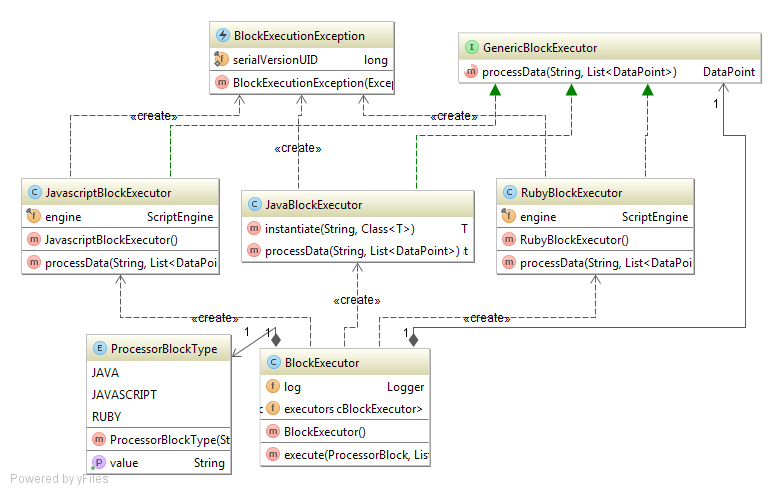
\includegraphics[width=1.3\textwidth, center]{blockExecutors}
		\caption{Diagrama claselor ce asigura executarea unei diagrame}
		\label{fig:blockExecutors}
	\end{figure}
	\item \code{JavascriptBlockExecutor}: Executor ce poate rula cod JavaScript pe server. Aceste blocuri trebuie să conţină o funcţie \code{parseInput} care ia ca parametru o listă de \code{DataPoint}. Pentru execuţia blocurilor de acest tip, standardul JSR 223 \autocite{JSR223} vine în ajutor prin abstractizarea funcţionalităţii interne necesare execuţiei de cod scris într-un limbaj dinamic, direct în maşina virtuală Java. În versiunea 8 a JVM-ului aceste funcţii sunt executate folosind runtime-ul de înaltă performantă Nashorn care este accelerat de modificări recente, introduse în JSR 292  \autocite{JSR292}, ridicând performanţa codului JavaScript la un nivel apropiat de funcţiile scrise în Java. Pentru versiunile precedente de JVM este folosit Mozilla Rhino. Dacă funcţia \code{parseInput} nu este găsită sau la execuţia script-uluiare loc o eroare, este generată o excepţie de tipul \code{BlockExecutionException}. Scriptul poate returna direct instanţe ale interfeţei \code{DataPoint}, sau alte obiecte care sunt apoi reprezentate ca un \code{StringDataPoint}.
	
	\item \code{RubyBlockExecutor}: Executor ce rulează cod Ruby pe server. Din punct de vedere al implementării este similar cu \code{JavascriptBlockExecutor}, însă foloseşte librăria JRuby \autocite{jruby} .
	
\end{itemize}

\section{Executarea unei diagrame funcţionale}
\Cref{fig:intrareDate} prezintă şi modul în care o diagrama este executată. Diagramele sunt lansate în execuţie de fiecare dată când un canal folosit în ea primeşte informaţii noi. Dacă două canale primesc date în acelaşi timp atunci diagrama va fi lansată în execuţie de două ori, câte o dată pentru fiecare punct de date primite.

\subsection{Ordinea execuţiei blocurilor}
Problema ordinii execuţiei unei FBD este intens dezbătută atât în literatură cât şi în aplicaţiile industriale. Cum standardul \textit{IEC61131-3} \autocite{IEC61131-3} nu propune o soluţie pentru ordinea de execuţie, producătorii industriali folosesc metode proprii, de la separarea blocurilor într-un tabel şi executarea de la stânga la dreapta, sus în jos \autocite[11]{TM241}, la definirea manuală a ordinii execuţiei \autocite[11]{Logix5000} sau folosind algoritmi care determina automat ordinea de execuţie \autocite[5]{GEFANUC}.

În implementarea din aplicaţia Alegria s-a ales proiectarea unei metode automate pentru depistarea ordinii în care diagrama trebuie executată. Deoarece aceasta reprezintă un graf aciclic orientat, prima etapă a execuţiei este transformarea într-un graf reprezentat prin lista de adiacenţă, unde fiecare bloc reprezintă un nod. Din această reprezentare se omit blocurile de comentarii. Odată ce transformarea a fost efectuată cu succes se încercă aplicarea unui algoritm de sortare topologică \autocite{toposort} a grafului obţinut. Aceasta implică găsirea unei ordini astfel încât pentru orice arc orientat $uv$ de la  $u$ la $v$, $u$ este înaintea lui $v$. 
Matematic problema poate fi formulata astfel:

\begin{definition} 
	O \textbf{ordine topologica}, notata $ord_D$, au unui graf orientat aciclic $D = (V,E)$ atribuie fiecărui nod o valoare astfel încât $ord_D(x) < ord_D(y)$ pentru orice arc $ x \rightarrow y \in E$.
\end{definition}
În literatura există mai mulţi algoritmi pentru efectuarea unei asemenea sortări \autocite{toposortArticle}, însă, deoarece grafurile în discuţie sunt statice, adăugându-se sau ştergându-se noduri, s-a ales un algoritm clasic, stabil din punct de vedere numeric descris de Kahn în 1962 \autocite{topoKahn}.

Simplificat, algoritmul implementat urmăreşte următorii paşi:
\begin{enumerate}
	\item Identifică toate nodurile spre care nu vine nici un arc. Valoarea acestor noduri va fi $0$. În cazul diagramelor, este vorba de toate canalele de intrare, şi de blocurile de procesare care nu au nici o intrare. Dacă aceste noduri nu există, înseamnă ca graful nu respecta condiţia de graf aciclic, deci acesta nu va putea fi executat;
	\item Se alege unul din nodurile găsite mai sus;
	\item Se şterge acest nod de valoare zero, împreună cu toate arcele care ies din el;
	\item Se repetă paşii 1 şi 2 până când nu mai există noduri în graf.
\end{enumerate}
Algoritmul descris mai sus rulează în $\mathcal{O}(V + E)$. 

\begin{algorithm}[H]
	\KwData{Un graf orientat acliclic reprezentat prin lista de adiacenţă}
	\KwResult{Lista nodurilor ordonate topologic}
	$L \gets$ Lista goală ce va conţine nodurile sortate \;
	$S \gets$ Lista tuturor nodurilor spre care nu există nici un arc \;
	\While{ $S$ conţine elemente }{ 
		şterge nodul $n$ din $S$ \;
		introdu nodul $n$ în $L$ \;
		\ForEach{nod $m$ care are un arc $e$ de la $n$ la $m$}{
			şterge arcul $e$ din graf\;
			\If{$m$ nu mai are arce spre el}
			{inserează $m$ în $S$}
		}{
	} 
	
}
\eIf{mai există arce în graf}
{\Return{\textbf{Eroare:} Graful are cel puţin un ciclu}}{
	{\Return{$L$ (graful sortat topologic)}}
}
\label{alg:khan}
\caption{Algoritmul lui Khan pentru sortare topologică}
\end{algorithm}

Astfel, pentru diagrama din \cref{fig:exempluDiagrama}, o posibilă ordine de execuţie este descrisă în \cref{fig:executionOrder}.
\begin{figure}[H]
	\centering
	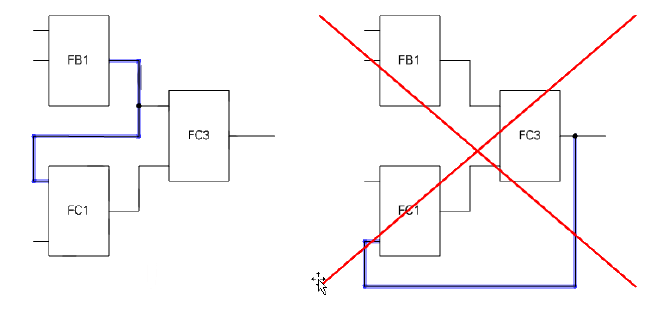
\includegraphics[width=0.95\textwidth]{badDiagram}
	\caption{Diagramă ce conţine cicluri}
	\label{fig:badDiagram}
\end{figure}

După cum se observă în \cref{alg:khan}, acesta poate detecta grafuri care conţin cicluri şi nu pot fi rezolvate. Această verificare permite detectarea erorilor, precum cea din diagrama \ref{fig:badDiagram} şi informarea utilizatorului pentru ca acesta să rezolve problema.

\begin{figure}[H]
	\centering
	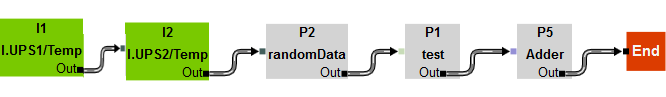
\includegraphics[width=\textwidth]{diagramExecutionOrder}
	\caption{Ordinea execuţiei pentru diagrama din \cref{fig:exempluDiagrama}}
	\label{fig:executionOrder}
\end{figure}

Deşi ciclurile la nivel de diagrama nu sunt permise, cele la nivel de canal sunt. Astfel, ieşirea unei diagrame poate fi setată ca intrare pentru aceeaşi diagramă, permiţând executarea în buclă, deoarece odată ce o diagrama se termină de executat şi salvează rezultatul pe canal, aceasta se relansează în execuţie cu noi informaţii. Cu astfel de bucle se pot implementa diagrame ce interacţionează între ele. Un alt aspect pozitiv al faptului ca ieşirile unor diagrame pot reprezenta intrări pentru alte diagrame este faptul că procese foarte complexe pot fi descompuse în părţile componente prin simpla înlănţuire a diagramelor.

\subsection{Generarea rezultatului}
Odată ce ordinea de execuţie a fost calculată, procesul de calcul al rezultatului este destul de simplu, fiind ilustrat în \cref{alg:executeDiagram}:

\begin{algorithm}[H]
	\KwData{Lista nodurilor ordonate topologic}
	\KwResult{Punctul de date ce trebuie adaugat pe canalul de iesire a diagramei}
	$rezultate \gets$ Relaţie cheie-valoare intre nod şi rezultatul execuţiei lui\;
	$L \gets$ Lista ce conţine nodurile sortate \;
	\ForEach{nod $m$ din $L$}{
		$intrari \gets$ Lista goala de intrări pentru nodul $m$ \;
		\ForEach{arc de la $n$ către $m$}{
			\eIf{In $rezultate$ exista rezultatul pentru blocul $n$}
			{Adaugă în $intrari$ valoarea de la $rezultate(n)$\;}{
				{\Return{\textbf{Eroare:} Graful nu poate fi executat\;}}
			}	
		}
		\eIf{$m$ este un bloc de procesare}
		{Executa blocul folosind intrările $intrari$\;
			Adaugă în $rezultate$ valoarea calculata\;}{
			\ElseIf{$m$ este un canal de date} {
				Adaugă în $rezultate$ ultima valoare de pe canal\;}
		} 
	}
	
	{\Return{Ultima valoare din $rezultate$}}
	\label{alg:executeDiagram}
	\caption{Execuţia unei diagrame FBD}
\end{algorithm}

\subsection{Implementarea execuţiei}
Pentru execuţia diagramelor este folosit Spring Bean-ul \code{DiagramExecutor}. Acesta este responsabil atât de parsarea unei diagrame cât şi de execuţia şi extragerea rezultatelor. Acest Bean poate fi apoi injectat folosind adnotarea \code{@Autowired} în toate clasele care doresc sa execute diagrame.

Parsarea este realizata cu ajutorul interfeţei \code{DiagramParser}, aceasta permiţând transformarea diagramei într-un graf reprezentat prin listă de adiacenţă. O implementarea a acestei interfeţe este clasa \code{GoJsDiagramParser} care parsează JSON-ul generat de librăria GoJS. Aceasta parsare se face cu ajutorul librăriei Jackson, folosind modelul de date din figura \cref{fig:gojsdiagramModel}. Dacă parsarea nu este realizata cu succes, atunci o excepţie de tipul \code{DiagramParseException} este aruncată.
Dacă se doreşte înlocuirea librăriei de front-end pentru realizarea diagramelor, sistemul poate fi adaptat doar prin scrierea unei noi clase ce implementează \code{DiagramParser}.

\begin{figure}[H]
	\centering
	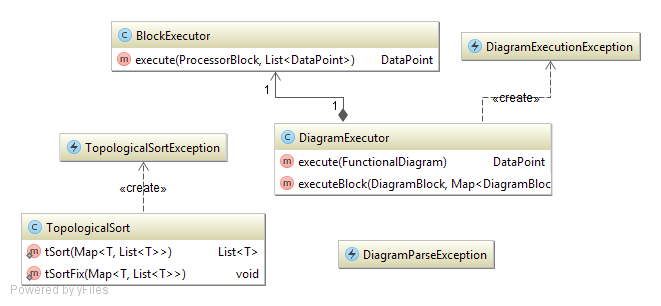
\includegraphics[width=\textwidth, center]{diagramExecuteClasses}
	\caption{Diagrama claselor implicate în executarea unei diagrame}
	\label{fig:diagramExecuteClasses}
\end{figure}
Odată ce parsarea a fost efectuată, execuţia blocului poate continua: folosind clasa \code{TopologicalSort}, o implementare a \cref{alg:khan} cu tipuri generice şi expresii lambda, ordinea de execuţie este calculată. Apoi, \cref{alg:executeDiagram} este executat, si, cu ajutorul bean-ului \code{BlockExecutor} blocurile din diagrama sunt executate. Rezultatul final al metodei \code{execute} este un \code{DataPoint} care va fi salvat în baza de date, pe canalul de ieşire a diagramei.

O alta chestiune importantă este determinarea momentelor când o diagrama trebuie executată. În acest scop, pe fiecare canal se stochează o mulţime de diagrame care trebuie lansate atunci când se primesc informaţii noi. Această listă este actualizată de fiecare data când diagrama se modifică prin interfaţa web. Metodele din \code{DiagramParser} sunt folosite pentru a obţine lista de canale utilizate şi pe fiecare dintre acestea, pe proprietatea \code{Set<FunctionalDiagram> subscribedDiagrams} este adăugată acea diagrama. Pentru a nu se pierde consitenţa datelor, cât timp diagrama este modificată, ea nu se mai poate lansa în execuţie.
\begin{figure}[H]
	\centering
	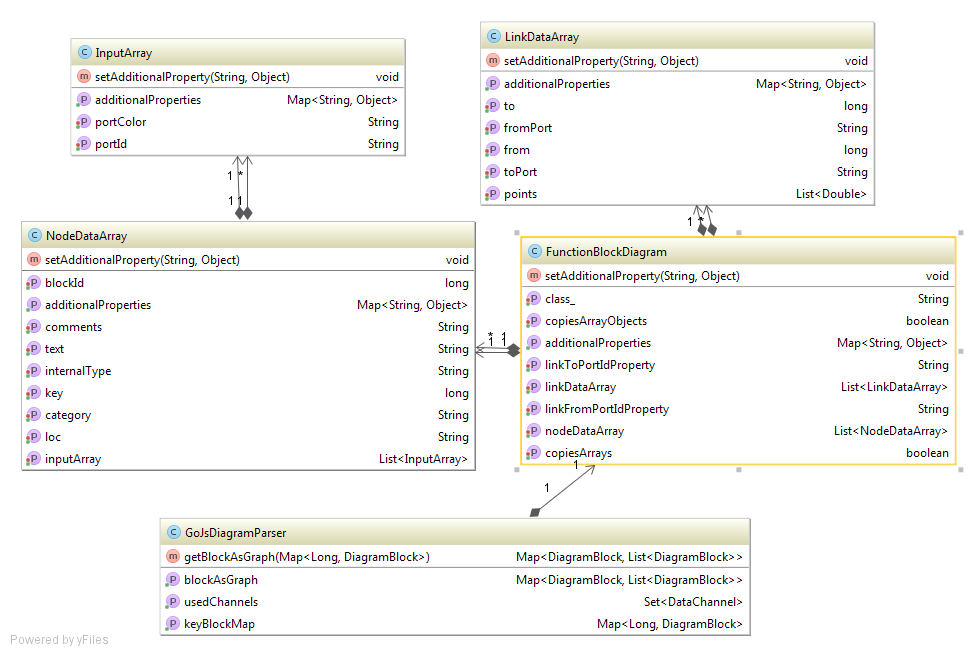
\includegraphics[width=1.2\textwidth, center]{gojsdiagramModel}
	\caption{Diagrama claselor ce reprezintă modelul de date pentru diagramele GoJS}
	\label{fig:gojsdiagramModel}
\end{figure}
\section{Serviciul de date}
Serviciul de date, implementat prin Spring Bean-ul \code{DataService} permite abstractizarea modului în care \code{DataPoint}-urile sunt scrise în baza de date. În această implementare, datele sunt stocate în aceeaşi instanta de PostgreSQL ca şi entităţile. Aceasta clasa foloseşte interogări SQL optimizate pentru a fi executate cat mai rapid, prin stocarea acestora direct pe serverul SQL.
\begin{figure}[H]
	\centering
	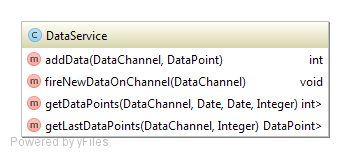
\includegraphics[width=0.6\textwidth, center]{dataService}
	\caption{Interfaţa aplicaţiei cu baza de date pentru informaţii}
	\label{fig:dataService}
\end{figure}
Această clasă asigură şi execuţia diagramelor din lista de \code{subscribedDiagrams} a canalului ce primeşte date. Această execuţie se executa în mod \textbf{asincron}, pentru a nu bloca firul de execuţie care primeşte date. Asincornicitatea este implementata printr-un pool de thread-uri care primesc task-uri de execuţie, thread-ul apelant nefiind interesat de rezultatul execuţiei. Astfel, putem considera că implementarea pe mai multe fire de execuţie este de tipul fire-and-forget.

Pentru a garanta o metoda de management a firelor de execuţie, s-au folosit capabilităţile native ale platformei Spring \autocite{springAsync} , prin adnotarea \code{@Async}.
\section{Baza de date}

După cum s-a discutat în capitolul despre arhitectura, aplicaţia are nevoie de mijloace de stocare pentru două tipuri de date: modelul entităţilor, şi datele primite şi procesate.
\subsection{Stocarea entităţilor} 
Petru stocarea entităţilor au fost investigate mai multe opţiuni de baze de date relaţionale, PostgreSQL fiind aleasă pentru stabilitatea şi posibilitatea de replicare volumelor mari de date, dar şi pentru uşurinţa extensibilităţii\autocite{postgresql}. Un alt avantaj al folosirii PostgreSQL este lipsa costului licenţei, întrucât este o aplicaţie open-source cu o comunitate foarte dinamică.
\begin{landscape}
	\begin{figure}
		\centering
		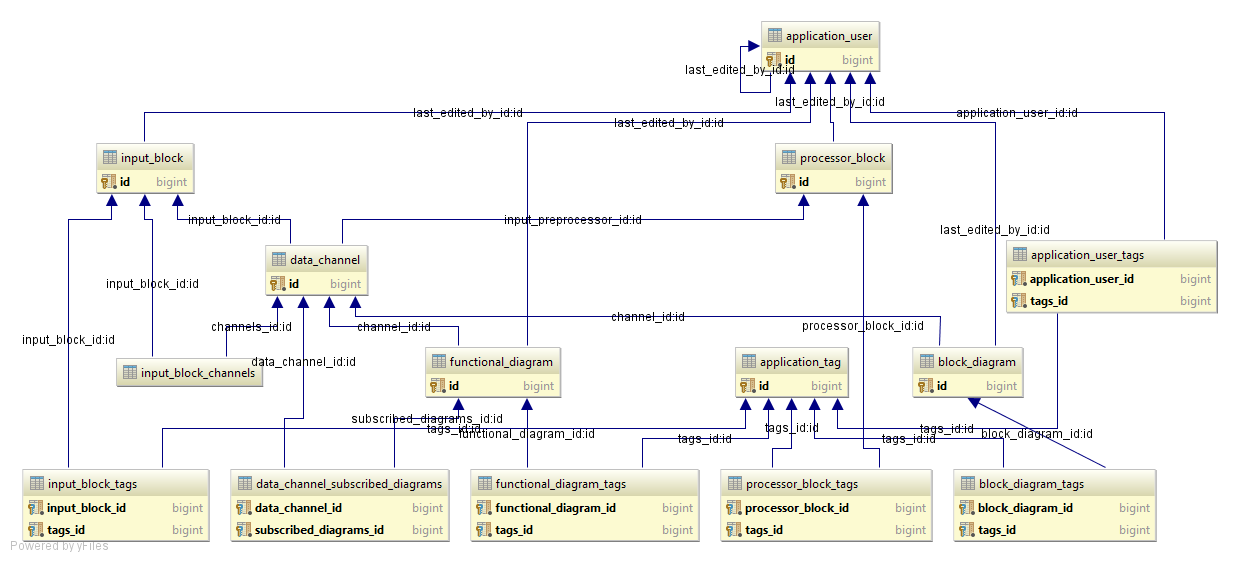
\includegraphics[width=1.8\textwidth]{dbDiagram}
		\caption{Modelul relaţional al entităţilor din baza de date}
		\label{fig:dbDiagram}
	\end{figure}
\end{landscape}

Pentru generarea schemei bazei de date s-a folosit ORM-ul implicit din Spring Data, Hibernate \autocite{hibernate} . Acesta permite generarea schema unei baze de date cu ajutorul programării orientate pe aspecte, prin adăugarea de adnotări pe clase Java. Această generare se realizează automat, de fiecare dacă când modelul Java se modifica.
\begin{figure}[H]
	\centering
	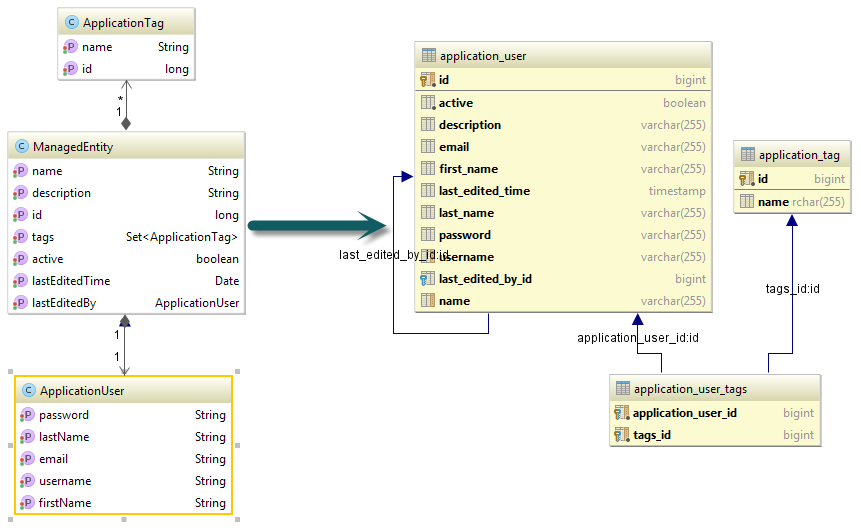
\includegraphics[width=\textwidth]{ORMtransform}
	\captionsetup{justification=centering}
	\caption{Transformarea claselor Java în relaţii din baza de date prin intermediul unui ORM}
	\label{fig:ORMtransform}
\end{figure} 

\chapter{Studiu de caz: Smart Home}



\chapter{Concluzii şi Dezvoltării ulterioare}
\label{chapter:concluzii}
\section{Concluzii}

Aceasta aplicaţie satisface cerinţa lumii moderne în care avem din ce în ce mai multe dispozitive inteligente, capabile sa se conecteze la diverse surse de date. În aceasta lume emergenta, serviciile sunt din ce în ce mai specializate, satisfăcând în mod complet o nişă. Orice persoana poate achiziţiona câţiva senzori inteligenţi, însă, pentru a obţine valoare din acei senzori, datele trebuie colectate, procesate şi stocate. 

Soluţia propusă răspunde astfel atât la problema colectării datelor din surse variate, cat şi la problema transformării acelor date în date utilizabile de alte sisteme, generând informaţii din date neprelucrate.

\section{Dezvoltării ulterioare}

Un aspect foarte important ce poate face scopul unei dezvoltării ulterioare este scalarea platformei într-o instantă cloud, ce poate fi folosita cu o arhitectura de tipul platform as a service (PaaS). Astfel, un utilizator poate externaliza serviciul de procesare a datelor, singura lui grijă fiind aducerea tuturor acelor date în sistem.

Împreună cu dezvoltarea de mai sus, o alta direcţie este alinierea cât mai bună cu conceptele din IoT (Internetul tuturor obiectelor). Aceasta aliniere s-ar putea realiza prin transformarea blocului de intrare în "thing"-uri, cu proprietăţi şi servicii. Tot în aceasta direcţie de dezvoltare s-ar putea include dezvoltarea de agenţi capabili sa interfaţeze între protocoale de date proprietare, şi soluţia propusă. Spre exemplu, implementarea unui client MQTT ar permite conectivitatea către o întreagă gama de dispozitive care respecta acest standard.

In vederea uşurării dezvoltării aplicaţiilor pe aceasta platforma trebuie suplimentat numărul de blocuri de procesare implicite existente în sistem.  

\printbibliography[title={Bibliografie}] % Change the title in the parenthes within the braces if you want

\end{document}